\documentclass[11pt]{report}
\usepackage[letterpaper, total={6.5in, 10in}]{geometry}
%\usepackage{fancyhdr}
%\pagestyle{fancy}
\usepackage{amsmath, amsthm, mathpazo, epic, eepic, color, array}
\usepackage{amssymb}
%\usepackage{graphicx}
\usepackage{cancel}
\usepackage{pgfplots}
\usepackage{multicol}
\pgfplotsset{compat=1.13}
\usepackage{etoolbox}
\makeatletter
\patchcmd{\chapter}{\if@openright\cleardoublepage\else\clearpage\fi}{}{}{}
\makeatother
\usepackage{hyperref}

\usepackage{enumerate}
\usepackage{enumitem}

\usepackage{tikz}
\usetikzlibrary{positioning,chains,fit,shapes,calc,arrows,patterns}
\usepackage{tkz-graph}
\usetikzlibrary{arrows, petri, topaths}
\usepackage{tkz-berge}
\usepackage[all]{xy}
\usepackage{textcomp}

\newboolean{colorprint}
\setboolean{colorprint}{true}
%\setboolean{colorprint}{false}

\ifthenelse{\boolean{colorprint}}{%
\newcommand{\colorone}{blue}
\newcommand{\colortwo}{red}
\newcommand{\coloronefill}{blue!15!white}
\newcommand{\colortwofill}{red!15!white}
\newcommand{\colormapone}{rgb=(.4,.4,1); rgb=(.8,.8,1)}
\newcommand{\colormaptwo}{rgb=(1,.4,.4); rgb=(1,.8,.8)}
\newcommand{\colormapplaneone}{rgb=(.7,.7,1); rgb=(.9,.9,1)}
\definecolor{colormaponebottom}{rgb}{.4,.4,1}
\definecolor{colormaponetop}{rgb}{.8,.8,1}
\definecolor{colormaptwobottom}{rgb}{1,.4,.4}
\definecolor{colormaptwotop}{rgb}{1,.8,.8}
}% ends color
{% not color
\newcommand{\colorone}{black}
\newcommand{\colortwo}{black!50!white}
\newcommand{\coloronefill}{black!15!white}
\newcommand{\colortwofill}{black!05!white}
\newcommand{\colormapone}{rgb=(.4,.4,.4); rgb=(.7,.7,.7)}
\newcommand{\colormaptwo}{rgb=(.6,.6,.6); rgb=(.9,.9,.9)}
\newcommand{\colormapplaneone}{rgb=(.8,.8,.8); rgb=(.95,.95,.95)}
\definecolor{colormaponebottom}{rgb}{.4,.4,.4}
\definecolor{colormaponetop}{rgb}{.7,.7,.7}
\definecolor{colormaptwobottom}{rgb}{.6,.6,.6}
\definecolor{colormaptwotop}{rgb}{.9,.9,.9}
}%

\newlength\tindent
\setlength{\tindent}{\parindent}
\setlength{\parindent}{0pt}
\renewcommand{\indent}{\hspace*{\tindent}}

\pgfplotsset{my style/.append style={axis x line=middle, axis y line=
middle, xlabel={$x$}, ylabel={$y$}, axis equal }}

\pgfplotsset{compat=1.13}

\usepackage[normalem]{ulem}

\begin{document}

{\bf Chapter 2: Derivatives}\\

%%%%%%%%%%%%%%%%%%%%%%Section 2.2%%%%%%%%%%%%%%%
{\bf Section 2.2 Interpretations of the Derivative}
\vskip .25 truein

All page numbers refer to original APEX text page numbers.\\
\\

\textbf{p. 72,} Example 41 last line change "$28,800 \cdot 156$" to "$(28,800)(156)$"\\ 


\textbf{p. 73} 2nd to last line (last line of last full paragraph) the $v(0)$ should $=52$ft/s.\\

\textbf{p. 74} \textbf{Inperpretation of ...Line} section 
\vskip .15 truecm
Last sentence of 1st paragraph. Delete "that intersects $f$ only once near $x=c$" 
\vskip .15 truecm
2nd to last line (last line of last full paragraph) the $v(0)$ should $=52$ft/s.\\
\vskip .5 truecm

\textbf{p. 77:  Exercises 2.2}
After \#18 insert the following exercises:

new \#19. If the tangent line to $y=f(x)$ at $(6,1)$ passes through the point $(2,4)$, find $f(6)$ and $f'(6)$.

new \#20. Sketch the graph of the function $f$ for which $f(0)=0, f'(0)>0, f'(1)=0,$ and $f'(3)<0$. 

new \#21. Sketch the graph of the function $h$ for which $h(1)=0, h'(1)>0, h'(2)=0,$ and $h'(3)>0$. 


\textbf{Answers} \vskip .25 truecm
19.   $f(6) = 1, f'(6)= -\frac{3}{4}$\vskip .25 truecm

20.   Answers vary. Possible solution \\

\begin{tikzpicture}
\begin{axis}[tick label style={font=\scriptsize},minor x tick num=1,axis y line=middle,axis x line=middle,ymin=-3,ymax=2,xmin=-.5,xmax=3.5,name=myplot, xscale=1/1,]
\addplot [domain=-0.5:3.5] {-x*(x-2)};
\end{axis}
\node [right] at (myplot.right of origin) {\scriptsize $x$};
\node [above] at (myplot.above origin) {\scriptsize $y$};
\end{tikzpicture}\\

\vskip .25 truecm
21.   Answers vary. Possible solution \\

\begin{tikzpicture}
\begin{axis}[tick label style={font=\scriptsize},minor x tick num=1,axis y line=middle,axis x line=middle,ymin=-2,ymax=2,xmin=0,xmax=3,name=myplot, xtick={1,2,3}, xticklabels={1,2,3}, xscale=.6/1,]
\addplot [domain=0:3] {(x-2)^3};
\end{axis}
\node [right] at (myplot.right of origin) {\scriptsize $x$};
\node [above] at (myplot.above origin) {\scriptsize $y$};
\end{tikzpicture}
\vskip 1 truecm

%%%%%%%%%%%%%%%%%%%%%%Section 2.3%%%%%%%%%%%%%%%
{\bf Section 2.3 Basic Differentiation Rules}
\vskip .25 truein

\textbf{p. 78}

Theorem 12 - Change format of way rules are listed. Put rule on same line as name \\
1. \textbf{Constant Rule:} $\displaystyle{\frac {d}{dx} (c)=0}$, \hskip 1.5 truein 2. \textbf{Power Rule:} $\displaystyle{\frac {d}{dx} (x^n) = nx^{n-1}}$ \\ \indent where $c$ is constant \hskip 2.2 truein where $n$ is any real number \vskip .25 truecm
and leave the rest of them as they are.\\

Change the discussion after the Theorem 12 box as follows:\\

Part 1 of this theorem states an intuitive fact: constant functions have \sout{no rate of change} a rate of change of zero, as they are constant. Therefore, their derivative is $0$ \sout{(they change at a rate of 0)}.  The proof is left as an exercise. \\

The theorem then states some amazing things. \\
In Part 2, the Power Rule states that the derivatives of \sout{Power Functions (} functions of the form $y=x^n$ where \textbf{$n$ is ANY real number} \sout{)} are very straightforward: multiply the power, then subtract $1$ from the power. This allows us to differentiate Power Functions, Root Functions, and functions with irrational exponents. The work we have done so far only allows us to prove the Power Rule when $n$ is a positive integer, which is presented here. We will provide proofs for other values of $n$ as we add the necessary tools to our knowledge of calculus.\\

\textbf{Proof: Differentiation Power Rule when $n$ is a positive integer}\vskip .25 truecm
Let $f(x)= x^n$, where $n \in \mathbb{Z}^+$. By the definition of derivative,\\
\small    %%%%%%  Changes text size - makes things fit better.%%%%%%%%%%%
\begin{flalign*}
\begin{aligned}
f'(x) &= \displaystyle{\lim_{h\to 0}} \frac{(x+h)^n - x^n}{h}, ~~\text{where}~ h \neq 0\\
&= \displaystyle{\lim_{h\to 0}} \frac{(x+h)^n - x^n}{h}, ~~\text{use the Binomial Theorem to expand\ } (x+h)^n\\  %%%Changed where this comment is and then there is only one align environment.  
&=\displaystyle{\lim_{h\to 0}} \frac{x^n + \binom{n}{1} hx^{n-1} + \binom{n}{2} h^2x^{n-2}+ ... +\binom{n}{n-1} h^{n-1}x + \binom {n}{n} h^n)   -x^n}{h},\\
&= \displaystyle{\lim_{h\to 0}} \frac{\binom{n}{1} hx^{n-1} + \binom{n}{2} h^2x^{n-2}+ ... +\binom{n}{n-1} h^{n-1}x + \binom {n}{n}  h^n}{h} \\
&= \displaystyle{\lim_{h\to 0}} \frac{\binom{n}{1} hx^{n-1} + \binom{n}{2} h^2x^{n-2}+ ... +\binom{n}{n-1} h^{n-1}x + \binom {n}{n}  h^n}{h} \\
&= \displaystyle{\lim_{h\to 0}} \frac{h[\binom{n}{1} x^{n-1} + \binom{n}{2} h x^{n-2}+ ... +\binom{n}{n-1} h^{n-2}x + \binom {n}{n} h^{n-1}]}{h},~~\text{we divide out}~h\\
&= \displaystyle{\lim_{h\to 0}}~ \binom{n}{1} x^{n-1} + \binom{n}{2} h x^{n-2}+ ... +\binom{n}{n-1} h^{n-2}x + \binom {n}{n} h^{n-1}, ~\text{since} \binom{n}{1} = n \\
&=  n x^{n-1}\\
\end{aligned}
\end{flalign*}
\normalsize  %%%%%Switch back to normal size.

\vskip .5 truecm

Theorem 12 part $3$ we proved in a previous section and part 4 is left as an exercise. In parts 5 and 6 we see something incredible about the functions $y=e^x$ and $y=\ln x$. We will use these rules freely, unfortunately their proofs will have to wait until we know a few more calculus techniques.\\

\textbf{Tim - we didn't discuss the "special case" of the Power Rule (i.e. $y=x^1$) as a group - I personally don't consider it a special case. It follows the rule just fine. I am inclined to cut this for now and ask later. What do you think?}
\vskip .5 truecm

\textbf{still on p. 79: Example 46} In the solution part 3 insert the work to take us from $(-1.1)^3 \approx 3(1.1-(-1))+(-1)=...$

\vskip .5 truecm

\textbf{On to p. 80}\\

Typo: 3rd line from the top - insert a "," between "sin x" and "nor".

\vskip .5 truecm
Insert proof of Sum Rule\\

\textbf{Proof: Sum Rule for Differentiation}\vskip .25 truecm
Let $f$ and $g$ be differentiable on an open interval $I$ and let $c$ be a real number,\\
\small
\begin{flalign*}
\begin{aligned}
\frac {d}{dx}( f(x) + g(x)) &= \lim_{h\to 0} \frac{[f(x+h)+g(x+h)] - [f(x)+g(x)]}{h}, ~~\text{where}~ h \neq 0\\
&= \lim_{h\to 0} \frac{[f(x+h)-f(x)] + [g(x+h) - g(x)]}{h}\\
&= \lim_{h\to 0} \frac{[f(x+h)-f(x)]}{h} + \lim_{h\to 0}\frac {g(x+h) - g(x)}{h}\\
&= f'(x) + g'(x)\\
\end{aligned}
\end{flalign*}
\normalsize
\vskip .5 truecm

Insert the following examples right before Example 47\vskip .25 truecm
Use Theorem 12 and 13 (or whatever they are now) to differentiate \vskip .25 truecm

1.  $g(x) = (x^2 + 1)^3$ \hskip 2 truecm 2. $f(x) = \ln \frac{\sqrt x}{8}$\vskip .25 truecm

SOLUTION
Given the differentiation rules we have thus far, our only option for finding $g'(x)$ is to first multiply $g(x)$ out and then apply the sum and power rules.\\

\begin{center} $g(x) = x^6 + 3x^4 + 3x^2 + 1$ \end{center}
thus, \\
\begin{center}$g'(x) = 6x^5 + 12x^3 + 6x$ \end{center}
\vskip .25 truecm

To differetiate $f(x)$ we will first need to use the Laws of Logarithms to expand $f$. 
\begin{flalign*}
\begin{aligned}
f(x) &= \ln \frac{\sqrt x}{8}\\
 &= \ln x^{\frac{1}{2}} - \ln 8 \\
&= {\frac{1}{2}}\ln x - \ln 8 \\
\end{aligned}
\end{flalign*}
so that,\\
\begin{center} $\displaystyle {f'(x) = {\frac{1}{2}} \cdot \frac{1}{x} -0 = \frac{1}{2x}}$ \end{center} 

\vskip 1.5 truecm


\textbf{p. 84:  Exercises 2.3}
Add the following problems:\\

new \#26 $h(x) = \frac{x^5-2x^3+x^2}{x^2}$\\

new \#27 $f(x) = \frac{x^2+1}{\sqrt x}$\\

new \#28 $g(\theta) = \frac{1-\sin^2 \theta}{\cos \theta}$\\

The current \#26 becomes \#29 then insert the following: \vskip .25 truecm


new \#30  Prove the Constant Rule: $\displaystyle{\frac {d}{dx} (c)=0}$, where $c$ is constant.\vskip .25 truecm

new\#31 The figure shows the graphs of $f, f',$ and $f''$. Identify each curve and explain your choices.\\

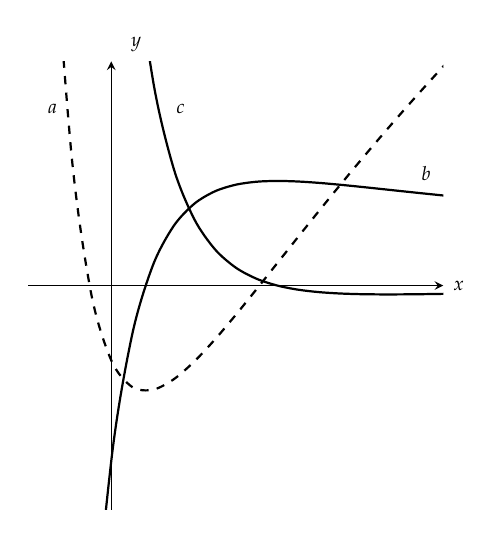
\begin{tikzpicture}
\begin{axis}[xtick=\empty, ytick=\empty, axis y line=middle,axis x line=middle, ymin=-3,ymax=3, xmin=-1,xmax=4, name=myplot, xscale=1/1.3,]
\addplot [{\colorone}, dashed, smooth, domain=-1:5,thick] {(6*(x^3-4*x)/((x+2)^3) +.65*x-1}; 
\node[label={30:{\scriptsize $a$}}] at (axis cs:-1,2.1) {};
\addplot [{\colortwo}, smooth, domain=-1:5,thick] {(13*x^3+78*x^2+876*x-376)/(20*x^3+120*x^2+240*x+160)};
\node[label={30:{\scriptsize $c$}}] at (axis cs:.55,2.1) {};
\addplot [{\colorone}, smooth, domain=-1:5, thick] {(-72*x+144)/(x^4+8*x^3+24*x^2+32*x+16)};
\node[label={30:{\scriptsize $b$}}] at (axis cs:3.5,1.2) {};
\end{axis}
\node [right] at (myplot.right of origin) {\scriptsize $x$};
\node [above] at (myplot.above origin) {\scriptsize $y$};
\end{tikzpicture}\\

new\#32 The figure shows the graphs of $f, f', f''$ and $f'''$. Identify each curve and explain your choices.\\

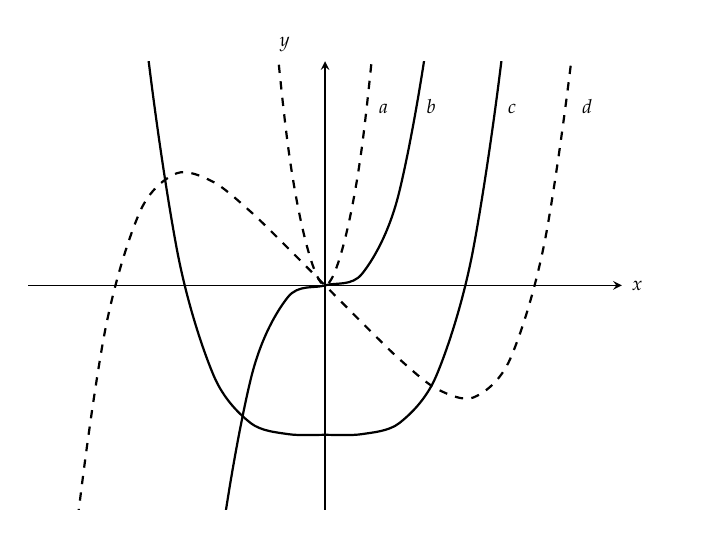
\begin{tikzpicture}
\begin{axis}[xtick=\empty, ytick=\empty, axis y line=middle,axis x line=middle, ymin=-3,ymax=3, xmin=-2,xmax=2, name=myplot, xscale=1.1/1,]
\addplot [{\colorone}, dashed, smooth, domain=-3:3,thick] {.5*x^5-2*x}; 
\node[label={30:{\scriptsize $a$}}] at (axis cs:.23,2.1) {};
\addplot [{\colortwo}, smooth, domain=-3:3,thick] {2.5*x^4-2};
\node[label={30:{\scriptsize $b$}}] at (axis cs:.55,2.1) {};
\addplot [{\colorone}, smooth, domain=-3:3, thick] {10*x^3};
\node[label={30:{\scriptsize $c$}}] at (axis cs:1.1,2.1) {};
\addplot [{\colortwo}, dashed, smooth, domain=-3:3, thick] {30*x^2};
\node[label={30:{\scriptsize $d$}}] at (axis cs:1.6,2.1) {};
\end{axis}
\node [right] at (myplot.right of origin) {\scriptsize $x$};
\node [above] at (myplot.above origin) {\scriptsize $y$};
\end{tikzpicture}
\vskip .5 truecm

The current \#27 - 32 become \#33 - 38 then insert the following: \vskip .25 truecm


new \#39. The position of a object is described by $s(t)=t^4 - 4t^2, t \geq 0$, where $s$ is in feet and $t$ is in seconds. Find\\
(a) the velocity and acceleration functions for the object,\\
(b) the acceleration after 1.5 seconds, and\\
(c) the time, in seconds, the object is at rest.
\vskip .25 truecm

new \#40. The position of a object is described by $s(t)=5e^t+5t$, where $s$ is in inches and $t$ is in seconds. Find\\
(a) the velocity and acceleration functions for the object,\\
(b) the acceleration after 2 seconds, and\\
(c) the acceleration when the object is at rest.\vskip .25 truecm

The current \#33 - 40 become \#41 - 48. \vskip .25 truecm


\vskip 1 truecm
\textbf{Answers}\\

26. $h'(x)=3x^2 - 2$\\

27. $f'(x)=\frac{3}{2}\sqrt x  - \frac{1}{2x \sqrt x}$\\ 

28. $g'(\theta)=-\cos \theta$\\ 


30.  $\displaystyle {\frac {d}{dx}(c) = \lim_{h\to 0} \frac{c - c}{h}=0, ~~\text{where}~ h \neq 0}$\vskip .25 truecm

31. $a$ is $f$, $b$ is $f'$, $c$ is $f''$
\vskip .25 truecm

32. $d$ is $f$, $c$ is $f'$, $b$ is $f''$, and $a$ is $f'''$
\vskip .25 truecm

39. (a) $v(t) = 4t^3 - 8t, ~ a(t)=12t^2 - 8$\\
\indent (b) $a(1.5) = 19~ \text{ft/s}^2$\\  
\indent (c) $t=0$ sec and $t=\sqrt{\frac{3}{2}}$ sec
\vskip .25 truecm

40. (a) $v(t) = 5e^x-5, ~ a(t)=5e^x$\\
\indent (b) $a(2) = 5e^2~ \text{ft/s}^2$\\  
\indent (c) $v(t)=0$ at $t=0$ sec, $a(0)=5~ \text{in/s}^2$ 

\end{document}